Dans cet exercice, toutes les questions et sous-questions sont, dans une large mesure, indépendantes. Certaines montent crescendo en difficulté. Toutes les réponses devront être argumentées.

\medskip
 
\noindent\begin{minipage}{.6\linewidth}
\begin{enumerate}
\item \textit{Une montre atypique.} 

Quand on regarde une montre du commerce et que la petite aiguille ajoute 12 (heures) à la position graduée sur 1 (heure), elle revient sur la position 1 (heure), comme dans le croquis ci-contre. En quelque sorte, \( 1 + 12 = 1 \).

Plutôt que de diviser la journée en 12 heures, on décide arbitrairement de la diviser en $n$ heures avec \( n \geqslant 2 \).

\begin{enumerate}
\item On choisit \( n = 5 \), croquis ci-contre. Justifier qu'en suivant le mouvement de la petite aiguille, on a \( 1 + 6 = 2 \). À quoi s'identifierait \( 1 + 12 \) ?

\item Comment choisir \( n \) de sorte que, cette fois, \( 1 + 12 = 2 \) ? Dessiner une horloge correspondante.
\end{enumerate}
\end{enumerate}
\end{minipage}
\hfill\begin{minipage}{.34\linewidth}
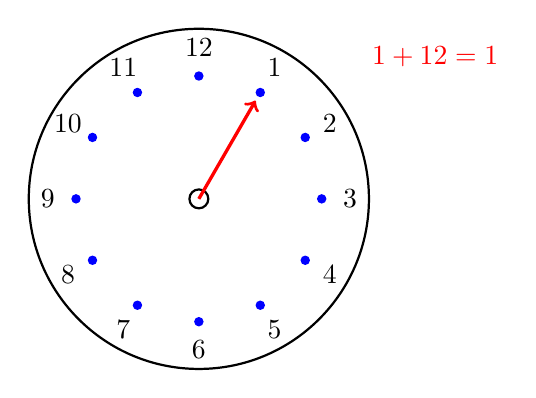
\begin{tikzpicture}[scale=1.2]
    % Cadre de l'horloge
    \draw[thick] (0,0) circle (1.8cm);
    \draw[thick] (0,0) circle (0.1cm);
    
    % Marques des heures
    \foreach \hour in {1,...,12} {
        \fill[thick,blue] (90-\hour*30:1.3cm) circle (0.05cm);
        \node at (90-\hour*30:1.6cm) { \hour};
    }
    
   
    
    % Aiguilles
    \draw[->,very thick, red] (0,0) -- (90-1*30:1.2cm); % Aiguille sur le 1

    
    % Équation en bas
    \node[red] at (2.5,1.5) { $1 + 12 = 1$};
\end{tikzpicture}

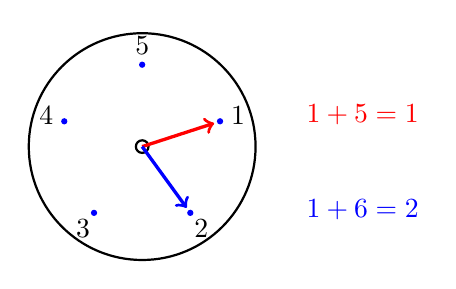
\begin{tikzpicture}[scale=.8]
    % Cadre de l'horloge
    \draw[thick] (0,0) circle (1.8cm);
    \draw[thick] (0,0) circle (0.1cm);
    
    % Marques des heures
    \foreach \hour in {1,...,5} {
        \fill[thick,blue] (90-\hour*360/5:1.3cm) circle (0.05cm);
        \node at (90-\hour*360/5:1.6cm) { \hour};
    }
    
   
    
    % Aiguilles
    \draw[->,very thick, red] (0,0) -- (90-1*360/5:1.2cm); % Aiguille sur le 1
    \draw[->,very thick, blue] (0,0) -- (90-2*360/5:1.2cm); % Aiguille sur le 2

    
    % Équation en bas
    \node[red] at (3.5,.5) { $1 + 5 = 1$};
        \node[blue] at (3.5,-1) { $1 + 6 = 2$};
\end{tikzpicture}
\end{minipage}


\begin{enumerate}
\setcounter{enumi}{1}
\item \textit{Traduction.} 

Exprimer ce que signifient les phrases suivantes (lues pratiquement telles quelles dans des médias !) :

\begin{enumerate}
\item « Il est indéniable que Beethoven n’aurait pas été le grand compositeur qu’il a été s’il n’avait pas été sourd » en utilisant le moins de négations possible.

\item « La mairie rejette la demande d'annulation déposée par l'association Organisons le premier Championnat de vitesse d'escargots I de l'arrêté municipal interdisant leur ramassage » en la remplaçant par deux ou trois phrases plus simples et plus claires montrant que vous l'avez bien comprise.
\end{enumerate}

\item\textit{Celle qui fait des mathématiques, c'est celle qui ne boit pas.} 

Une coupe de champagne conique est remplie à ras bord. Mais la personne à qui la coupe est destinée n'en veut pas. Elle la vide dans d'autres coupes initialement vides et identiques, en les remplissant chacune jusqu'à la moitié de leur hauteur $h$.

 Combien de coupes remplit-elle ainsi ?


\end{enumerate}

% Illustration des coupes (simplifiée)
\begin{tikzpicture}[scale=1.2]

% Pied de la coupe
\fill[gray!75, blur shadow] (0,0) ellipse (0.5 and 0.15);
%\fill[gray!70] (-0.5,0) .. controls (-0.5,0.2) and (-0.4,0.8) .. (-0.25,.3) 
                -- (0.25,1.2) .. controls (0.4,0.8) and (0.5,0.2) .. (0.5,0) -- cycle;

% Tige fine
\fill[gray!65] (-0.08,0) rectangle (0.08,2.8);

% Base du cône
\fill[blue!70] (0,2.8) ellipse (0.25 and 0.08);

% Verre conique - extérieur
\fill[white!95!blue, opacity=0.8]     (0,2.8) ellipse (0.25 and 0.08)    -- (-1.2,5.0)    -- (1.2,5.0) -- cycle;

% Bord du verre
\draw[very thick, white!80!gray] (-1.2,5.0) -- (1.2,5.0);



% Liquide champagne (surface horizontale)
\fill[yellow!50!white, opacity=0.7] 
    (-0.,2.8) -- (1.2,5) -- (-1.2,5) -- cycle;



% Hauteur h avec flèche
\draw[<->, line width=1pt, gray!50] (1.6,2.8) -- (1.6,5.0);
\draw[line width=1pt, gray!50] (1.5,2.8) -- (1.7,2.8);
\draw[line width=1pt, gray!50] (1.5,5.0) -- (1.7,5.0);
\node[text=gray!90, right] at (1.8,3.9) {\large $h$};

\end{tikzpicture} $=$
\begin{tikzpicture}[scale=1.2]

% Pied de la coupe
\fill[gray!75, blur shadow] (0,0) ellipse (0.5 and 0.15);
%\fill[gray!70] (-0.5,0) .. controls (-0.5,0.2) and (-0.4,0.8) .. (-0.25,.3) 
                -- (0.25,1.2) .. controls (0.4,0.8) and (0.5,0.2) .. (0.5,0) -- cycle;

% Tige fine
\fill[gray!65] (-0.08,0) rectangle (0.08,2.8);

% Base du cône
\fill[blue!70] (0,2.8) ellipse (0.25 and 0.08);

% Verre conique - extérieur
\fill[white!95!blue, opacity=0.8]     (0,2.8) ellipse (0.25 and 0.08)    -- (-1.2,5.0)    -- (1.2,5.0) -- cycle;

% Bord du verre
\draw[very thick, white!80!gray] (-1.2,5.0) -- (1.2,5.0);



% Liquide champagne (surface horizontale)
\fill[yellow!50!white, opacity=0.7] 
    (-0.,2.8) -- (.6,3.9) -- (-.6,3.9) -- cycle;



% Hauteur h avec flèche
\draw[<->, line width=1pt, gray!50] (1.6,2.8) -- (1.6,3.9);
\draw[line width=1pt, gray!50] (1.5,2.8) -- (1.7,2.8);
\draw[line width=1pt, gray!50] (1.5,3.9) -- (1.7,3.9);
\node[text=gray!70, right] at (1.8,3.35) {\large $\dfrac{h}{2}$};
\end{tikzpicture}$+$\begin{tikzpicture}[scale=1.2]

% Pied de la coupe
\fill[gray!75, blur shadow] (0,0) ellipse (0.5 and 0.15);
%\fill[gray!70] (-0.5,0) .. controls (-0.5,0.2) and (-0.4,0.8) .. (-0.25,.3) 
                -- (0.25,1.2) .. controls (0.4,0.8) and (0.5,0.2) .. (0.5,0) -- cycle;

% Tige fine
\fill[gray!65] (-0.08,0) rectangle (0.08,2.8);

% Base du cône
\fill[blue!70] (0,2.8) ellipse (0.25 and 0.08);

% Verre conique - extérieur
\fill[white!95!blue, opacity=0.8]     (0,2.8) ellipse (0.25 and 0.08)    -- (-1.2,5.0)    -- (1.2,5.0) -- cycle;

% Bord du verre
\draw[very thick, white!80!gray] (-1.2,5.0) -- (1.2,5.0);



% Liquide champagne (surface horizontale)
\fill[yellow!50!white, opacity=0.7] 
    (-0.,2.8) -- (.6,3.9) -- (-.6,3.9) -- cycle;



% Hauteur h avec flèche
\draw[<->, line width=1pt, gray!50] (1.6,2.8) -- (1.6,3.9);
\draw[line width=1pt, gray!50] (1.5,2.8) -- (1.7,2.8);
\draw[line width=1pt, gray!50] (1.5,3.9) -- (1.7,3.9);
\node[text=gray!90, right] at (1.8,3.35) {\large $\dfrac{h}{2}$};
\end{tikzpicture}$+\qquad\overset{?}\dots$
\newpage
\begin{enumerate}
\setcounter{enumi}{3}
\item \textit{Ou alors juste un peu.} 

Un verre est formé par une demi-sphère (représentée en coupe par un demi-cercle sur le dessin). Le verre est rempli jusqu'à la moitié de sa hauteur \( h \). Quel est l'angle d'inclinaison maximum \( x \) selon lequel on peut pencher ce verre sans renverser de liquide ?


\end{enumerate}

\begin{center}
\begin{tikzpicture}[scale=1.5]
% Liquide (remplissage à moitié)
\draw[thick,blue!30,  fill=blue!30, opacity=0.6] (1.3,3.55) arc (-30:-150:1.5cm) -- cycle;
\draw[dashed] (1.3,3.55) -- (1.6,3.55) ;
\draw[dashed] (1.6,2.8) -- (-1.6,2.8) ;

% Pied de la coupe
\fill[gray!75,] (0,0) ellipse (0.5 and 0.15);

% Tige fine
\fill[gray!65] (-0.08,0) rectangle (0.08,2.8);

% Base du cône
\fill[blue!30] (0,2.8) ellipse (0.25 and 0.08);

% Paroi arrière (en pointillés)
\draw[thick] (1.5,4.3) arc (0:-180:1.5cm);

%% Hauteur h avec flèche
\draw[<->, line width=1pt, black!70] (1.6,2.8) -- (1.6,3.55);
\draw[line width=1pt, black!70] (1.5,2.8) -- (1.7,2.8);
\draw[line width=1pt, black!70] (1.5,3.55) -- (1.7,3.55);
\node[text=black!70, right] at (1.6,3.17) { $\dfrac{h}{2}$};

\draw[<->, line width=1pt, black!70] (-1.6,2.8) -- (-1.6,4.3);
\draw[line width=1pt, black!70] (-1.5,2.8) -- (-1.7,2.8);
\draw[line width=1pt, black!70] (-1.5,4.3) -- (-1.7,4.3);
\node[text=black!70, right] at (-2,3.55) { $h$};
\end{tikzpicture}\hfil 	
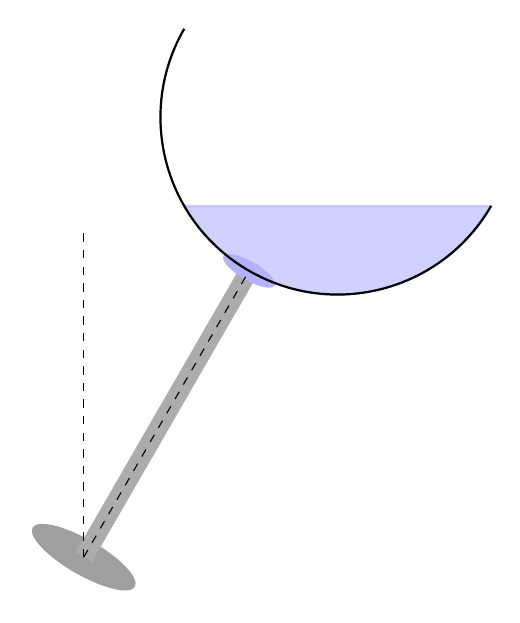
\begin{tikzpicture}[scale=1.5,rotate around={-30:(0,4.3)}]
% Liquide (remplissage à moitié)
\draw[thick, blue!30, fill=blue!30, opacity=0.6,rotate around={30:(0,4.3)}] (1.3,3.55) arc (-30:-150:1.5cm) -- cycle;

% Pied de la coupe
\fill[gray!75,] (0,0) ellipse (0.5 and 0.15);

% Tige fine
\fill[gray!65] (-0.08,0) rectangle (0.08,2.8);

% Base du cône
\fill[blue!30] (0,2.8) ellipse (0.25 and 0.08);

% Paroi arrière (en pointillés)
\draw[thick] (1.5,4.3) arc (0:-180:1.5cm);

\draw[dashed,rotate around={30:(0,0)}] (0,0) -- (0,2.8) ;
\draw[dashed] (0,0) -- (0,2.8) ;

\end{tikzpicture}
\end{center}

\begin{enumerate}
\setcounter{enumi}{4}

\item \textit{Mais les mathématiciens ont le droit de manger.} 

Un groupe d'une centaine de personnes réserve un dîner dans un restaurant niçois avec vue sur mer. En temps normal, le prix du repas est de 40 euros par personne. Mais le gérant exige que sa recette (c'est-à-dire le total de ce que le groupe payera) atteigne au minimum 4 000 euros, ceci afin de couvrir les risques qu'il prend en leur réservant les tables si trop de convives se désistent.

\begin{enumerate}
\item Justifier que, si \( n \geqslant 100 \) personnes viennent, elles payeront bien 40 euros chacune, mais que si, du fait de défections, seulement \( n < 100 \) personnes viennent, elles payeront alors davantage chacune. Combien paye chacun lorsque seulement 90 personnes viennent ?

\item Le groupe obtient une subvention de 1 000 euros de l'État. Combien paye chacun lorsque seulement 90 personnes viennent ? Lorsque 120 personnes viennent ? Combien de personnes doivent venir, exactement, pour que le prix que chacun paye soit minimal ?
\end{enumerate}

\noindent\begin{minipage}{.65\linewidth}
\item \textit{Et de prendre un dessert.} 

Soit une portion de tarte représentée par le secteur angulaire ayant la forme d’un quart de disque (l’ouverture angulaire vaut \( \dfrac{\pi}{2} \)). On souhaite la diviser en deux parties égales. Mais d’une manière originale : en la coupant non pas le long de son axe de symétrie, mais le long d’une perpendiculaire à cet axe, dessin ci-contre. Ainsi, l’aire du morceau de gauche serait égale à l’aire du morceau de droite. Où faut-il couper ? (On introduira toutes les variables nécessaires à la résolution de ce problème.)
\end{minipage}
\hfill\begin{minipage}{.35\linewidth}
\begin{center}
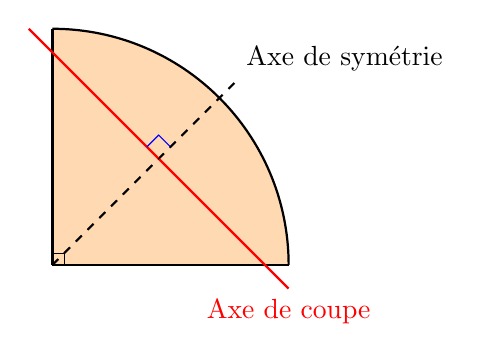
\begin{tikzpicture}[scale=1.5]

% Quart de disque
\fill[orange!30] (0,0) -- (2,0) arc (0:90:2cm) -- cycle;
\draw[thick] (0,0) -- (2,0);
\draw[thick] (0,0) -- (0,2);
\draw[thick] (2,0) arc (0:90:2cm);

% Axe de symétrie (en pointillés)
\draw[dashed, thick] (0,0) -- (45:2.2cm) node[above right] {Axe de symétrie};

% Axe de coupe (perpendiculaire)
\draw[red, thick] (-0.2,2) -- (2,-.2) node[below] {Axe de coupe};
%\draw[red, thick, ->] (0.23,1.46) -- (0.33,1.56);

% Angle droit
\draw[thin, blue] (1,1) -- (0.9,1.1) -- (0.8,1);
\draw[thin, black] (0,.1) -- (0.1,.1) -- (0.1,0);

% Rayon
\draw[thin, dashed] (0,0) -- (1.414,1.414);

\end{tikzpicture}
\end{center}
\end{minipage}





\noindent\begin{minipage}{.65\linewidth}
\item \textit{Pythagore 3D (théorème de de Gua).} 

Montrer que, dans un tétraèdre trirectangle (trois angles droits en un sommet), c'est-à-dire un coin de parallélépipède rectangle, le carré de l'aire de la face oblique est égal à la somme des carrés des aires des trois autres faces.

\end{minipage}
\hfill\begin{minipage}{.35\linewidth}
\tdplotsetmaincoords{70}{110}
\begin{tikzpicture}[tdplot_main_coords, scale=1.5]

% Coordonnées des points
\coordinate (O) at (0,0,0);
\coordinate (A) at (3,0,0);
\coordinate (B) at (0,2,0);
\coordinate (C) at (0,0,2);

% Faces rectangles
\fill[blue!20, opacity=0.6] (O) -- (A) -- (C) -- cycle; % Face OAC
\fill[green!20, opacity=0.6] (O) -- (B) -- (C) -- cycle; % Face OBC
\fill[red!20, opacity=0.6] (O) -- (A) -- (B) -- cycle; % Face OAB

% Face oblique ABC
\fill[yellow!30, opacity=0.7] (A) -- (B) -- (C) -- cycle;

% Arêtes
\draw[thick] (O) -- (A) node[midway,right] {$a$};
\draw[thick] (O) -- (B) node[midway,above] {$b$};
\draw[thick] (O) -- (C) node[midway,left] {$c$};

% Arêtes de la face oblique
\draw[thick] (A) -- (B);
\draw[thick] (B) -- (C);
\draw[thick] (C) -- (A);

% Angles droits
\draw[thin] (0.3,0,0) -- (0.3,0.2,0) -- (0,0.2,0);
\draw[thin] (0,0,0.2) -- (0.3,0,0.2) -- (0.3,0,0);
\draw[thin] (0,0.2,0) -- (0,0.2,0.2) -- (0,0,0.2);

% Labels
\node[below] at (A) {$A$};
\node[right] at (B) {$B$};
\node[above] at (C) {$C$};
\node[above left] at (O) {$S$};

% Annotation des aires
%\node[blue] at (1.5,0,1) {Aire $= \frac{1}{2}ac$};
%\node[green] at (0,1,1) {Aire $= \frac{1}{2}bc$};
%\node[red] at (1.5,1,0) {Aire $= \frac{1}{2}ab$};
%\node[above] at (1.5,1,1.5) {Aire $= \frac{1}{2}\sqrt{a^2b^2 + b^2c^2 + c^2a^2}$};

\end{tikzpicture}
\end{minipage}

\end{enumerate}
